\documentclass[../Main.tex]{subfiles}

\begin{document}
\author{Photoelectric Effect} %use author for title of lesson
\date{Year 1 Topic 20} %use date to refer to topic in main booklet

\section{Photoelectric Effect} %Section is the title of the lesson repeated, ready for the main contents page.

\begin{frame}{Light as a particle}
\begin{multicols}{2}
\begin{minipage}{7cm}
   So we have now seen light as being packets of energy taking on quantised values, $E=hf$ -- what were the symbols and their units?
   \pause
   \begin{itemize}
       \item h = Planck constant = $6.63\times 10 ^{-34}$Js
       \item f = frequency of EM wave in Hz
   \end{itemize}
   This usually means that a photon has a very small amount of energy, so we often use the electronvolt (eV) as an alternative.
   \end{minipage}
   \pause

   \begin{exampleblock}{Quick Calculation}
   Determine the energy in eV of a photon of a radio wave with a frequency of 96.5MHz. \pause 
   -- 0.4$\mu$eV.
   \end{exampleblock} \pause
  
   \columnbreak
   \begin{figure}
       \centering
       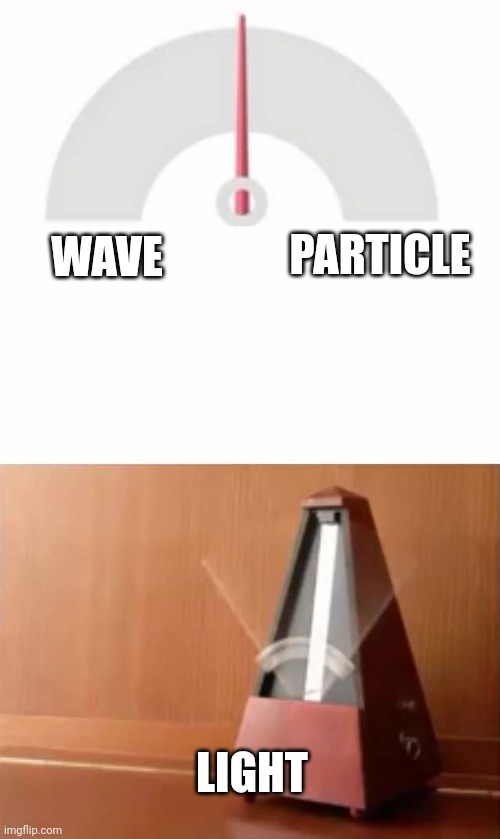
\includegraphics[height=3.5cm]{Quantum_Images/lightwaveparticle.jpg}
   \end{figure}
   \end{multicols}
Of course with all this, light still shows wave behaviours as we have seen previously - diffraction, refraction, reflection, interference, etc.
\end{frame}

\begin{frame}{A bit of History}
\begin{multicols}{2}
Around 1905, Einstein investigated an unexplained phenomenon known as the photoelectric effect, which was discovered almost 20 years before by Heinrich Hertz -- yes the same Hertz for the unit!
\pause
\begin{minipage}{6cm}
\begin{block}{Light and electrons?}
Hertz found that when UV light was incident upon a negatively charged gold surface, the surface lost its charge. The implication of this was that the UV light caused electrons to be emitted from the metal. Upon trying this for lower frequency light, the effect was not observed.
\end{block}
\end{minipage}
\columnbreak
    \begin{figure}
        \centering
        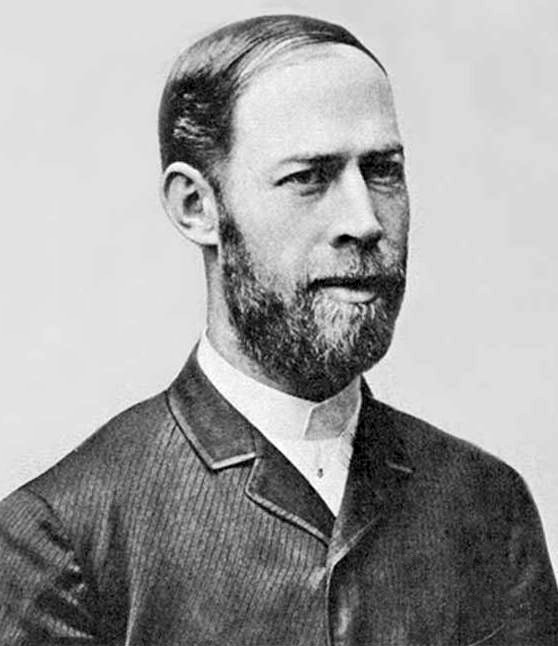
\includegraphics[width=3cm]{Quantum_Images/Heinrich_Rudolf_Hertz.jpg}
    \end{figure}
    \begin{figure}
        \centering
        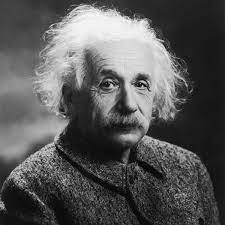
\includegraphics[width=3cm]{Quantum_Images/einstein.jpeg}
    \end{figure}
    \end{multicols}
\end{frame}

\begin{frame}{Photoelectric effect}
    Some important things were noticed about the photoelectric effect:
    \begin{itemize}
        \item Below certain frequencies of light, no electrons were emitted \pause
        \item The intensity of light did not affect if electrons were emitted (i.e for a lower frequency nothing still happened) \pause
        \item When above a certain frequency, increasing the intensity of light only meant more electrons were emitted \pause
        \item Photoemission is instantaneous
        \end{itemize}
        
    \pause
    This was explained by Einstein in the form of photons:
    \begin{itemize}
        \item electrons are emitted on a 1:1 basis to photons, i.e. 1 photon caused 1 electron to be emitted. Thus increasing the intensity meant more photons and so more electrons. \pause
        \item The minimum frequency means that electrons need a minimum amount of energy to be emitted, obtained using $E=hf$
    \end{itemize}
    
    PhET sim -- \url{https://phet.colorado.edu/en/simulations/photoelectric}
\end{frame}

\begin{frame}{Evidence against light as a wave}
    If instead we look at the wave nature of light, this evidence contrasts to wave theory, where it would be expected that the frequency of light would not matter. 
    \newline 
    
    \newline
    The energy transfer, being continuous, would build up until enough energy is collected for an electron to be emitted. So there would also be a time delay between incidence and emission. Or alternatively, increasing the intensity of light would add more energy faster. 
    \newline
    
    \newline
    But these effects are not what is observed. Wave theory of light fails to explain the photoelectric effect, but the photon model does, so therefore light can be explained as a particle as well.
\end{frame}

\begin{frame}{Photoelectric effect}
    \begin{block}{Photoelectric effect}
        When photons of a frequency above a minimum value are incident upon a metal surface, electrons are emitted. 
    \end{block}
    
    \begin{itemize}
        \item This frequency we call the threshold frequency, $f_0$
        \item The electrons are also known as photoelectrons -- they are still actual electrons, but their origin is described in the name.
    \end{itemize}
    
    \begin{figure}
        \centering
        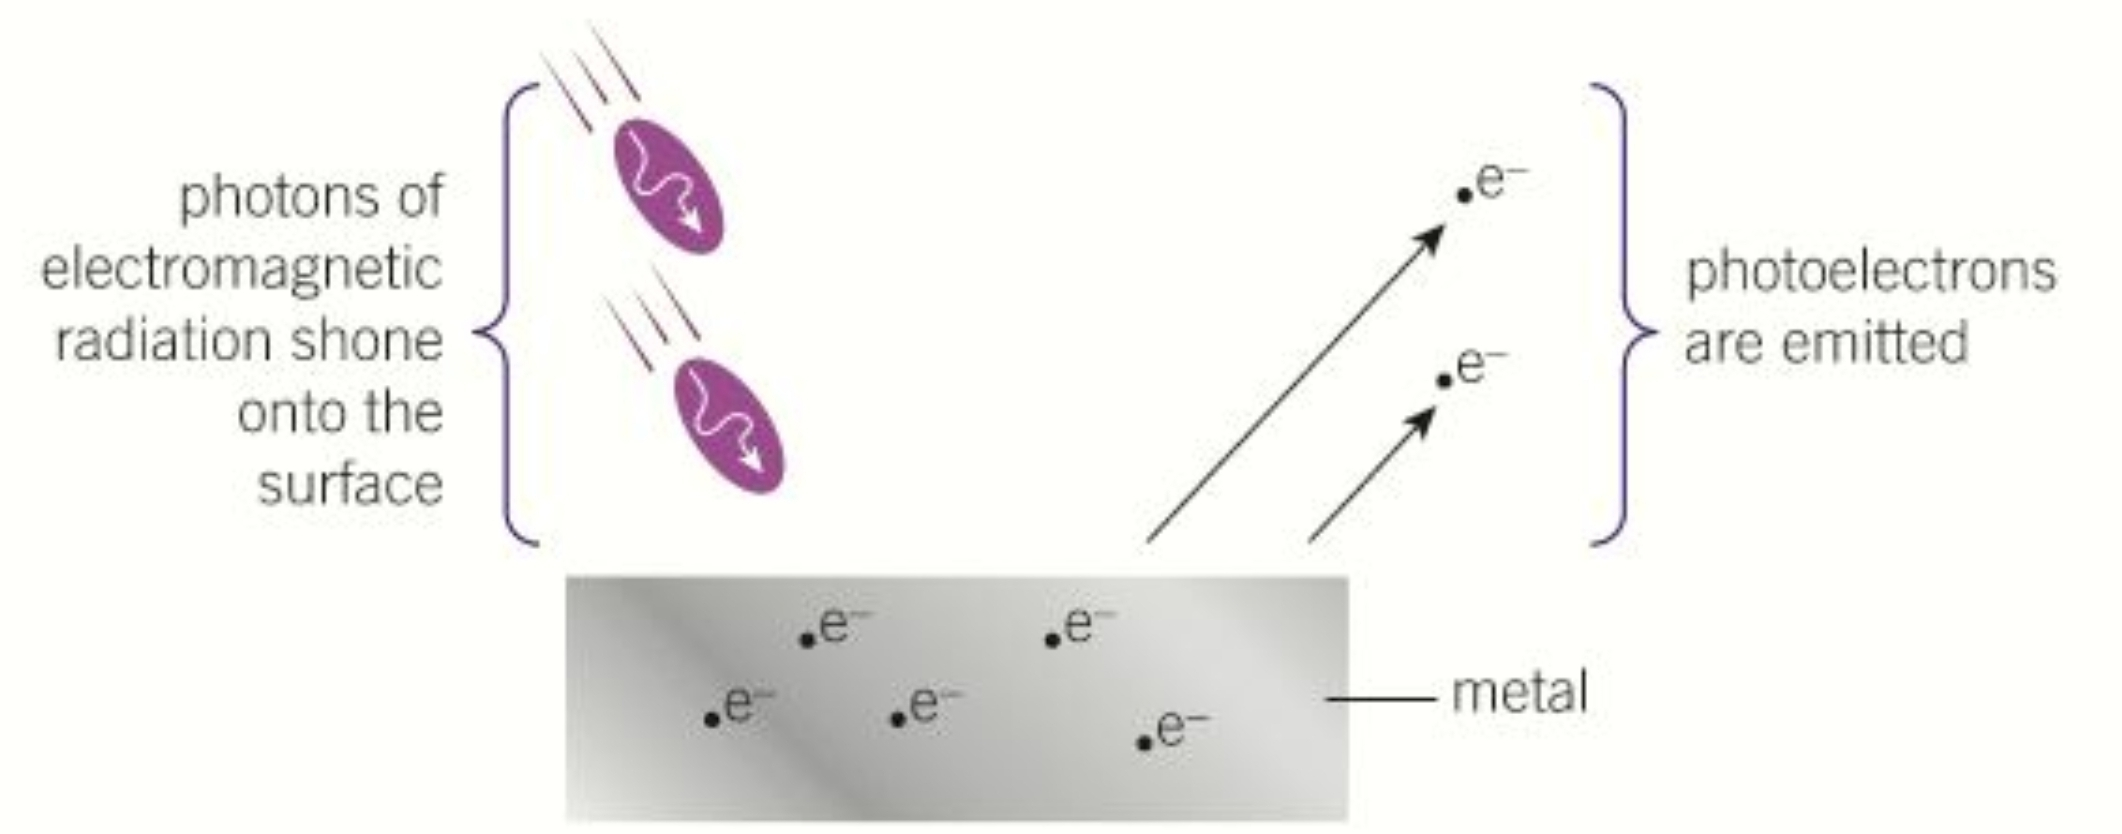
\includegraphics[width=0.8\textwidth]{Quantum_Images/photoelectrons.jpg}
    \end{figure}
\end{frame}

\begin{frame}{Photoelectric effect equation}
    The minimum amount of energy per photon required to emit a photoelectron is called the \emph{work function}, denoted $\phi$, and is unique to every metal surface
    \begin{equation*}
        hf = \phi 
    \end{equation*}
    But that's only the minimum... what might happen if a photon has \emph{more} energy than the minimum? Due to conservation of energy that extra energy must go somewhere... \pause
    
    \begin{block}{The extra energy}
    The extra energy is given to the electron in the form of kinetic energy
    \end{block}
    \begin{equation*}
        hf = \phi + KE_{max}
    \end{equation*}
    Note that $hf$ is the energy photon in Joules, $\phi$ is the work function in Joules, and $KE_{max}$ is also in Joules.
\end{frame}

\begin{frame}{Examples}
    \begin{exampleblock}{Example 1}
    The work function for lithium is $4.6 \times 10^{-19}$ J. \newline
a) Calculate the lowest frequency of light that will cause photoelectric emission. \pause 
-- $6.9\times10^{14}$Hz \newline 
b) What is the maximum energy of the electrons emitted when light of $7.3\times 10^{14}$ Hz is used? \pause
-- $2.6\times10^{-20}$ J (0.17eV)
    \end{exampleblock} 
    So long as the energy of the photon, the work function, and the kinetic energies are all given in eV, we can use $E=\phi+EK_{max}$
    
    \begin{exampleblock}{Example 2}
    Aluminium has a work function 4.08eV. Calculate the maximum kinetic energy of photoelectrons emitted when aluminium is illuminated with photons of \newline a) 5.20eV \pause 
    -- 1.12eV
    \newline b) 3.10eV \pause 
    -- photoelectrons are not emitted
    \end{exampleblock}
\end{frame}

\begin{frame}{Why maximum?}
    \begin{equation*}
        hf = \phi + EK_{max}
    \end{equation*} 
    Why is this a maximum kinetic energy? \pause
    \begin{figure}
        \centering
        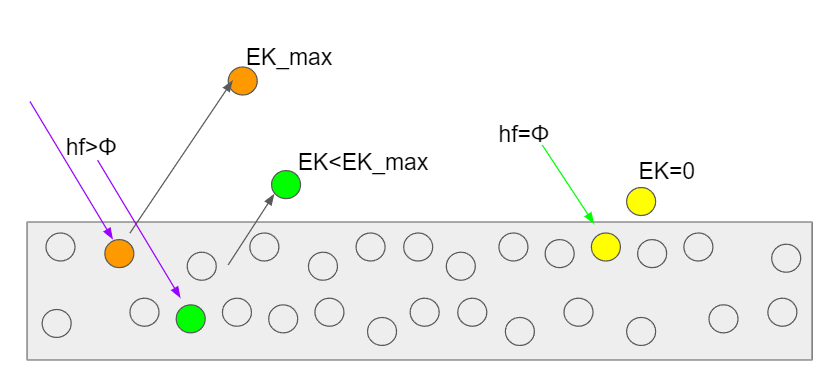
\includegraphics[height=3.5cm]{Quantum_Images/maxkineticenergy.png}
    \end{figure}
    The work function is the energy required to \emph{just} release an electron from right on the surface. With higher energy photons, the maximum kinetic energy electrons come from right on the surface too. Electrons below the surface will therefore have less kinetic energy
\end{frame}

\begin{frame}{Graphical representations}
    If we plot a graph of frequency against electron kinetic energy, we would rearrange the formula to become $EK_{max}=hf-\phi$ -- what would the gradient and y-intercepts be? Might there be an x-intercept? \pause
    
    \begin{figure}
    \begin{subfigure}
        \centering
        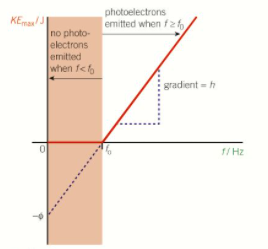
\includegraphics[height=4cm]{Quantum_Images/photoelectriceffectgraph.png}
        \end{subfigure}
        \pause
        \begin{subfigure}
        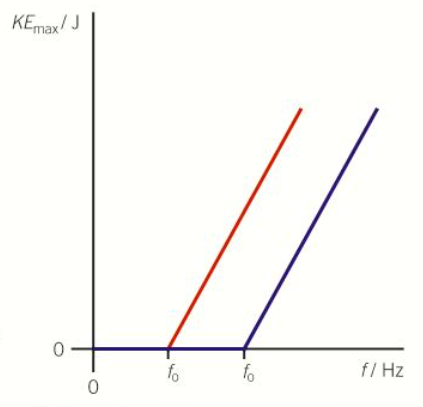
\includegraphics[height=4cm]{Quantum_Images/photoelectriceffect_differentmetals.png}
        \end{subfigure}
    \end{figure}
    Since different metals have different work functions, they have different threshold frequencies, but the gradient will still be the same -- Planck's constant is constant!
\end{frame}
\end{document}